\section{Pendahuluan}
\subsection{Latar Belakang}
Perkembangan teknologi jaringan komputer sudah menjadi tulang punggung bagi komunikasi di era modern ini, baik dari skala kecil maupun dalam skala besar. Dua aspek penting dalam mendukung konektivitas sekarang ini adalah Crimping dan juga Routing IPv4. Crimping sendiri merupakan proses fisik dalam menghubungkan kabel jaringan dengan memastikan bahwa koneksi fisik yang stabil dan minim gangguan, sedangkan Routing IPv4 merupakan proses dalam mengarahkan paket data melalui jaringan berdasarkan alamat IP dengan tujuan data mencapai tujuan yang tepat melalui berbagai perangkat jaringan seperti router.

\subsection{Dasar Teori}
\subsubsection{Crimping}
Crimping adalah proses yang menyambungkan kabel UTP ke konektor dengan menggunakan alat crimping untuk mendukung transmisi data yang stabil dalam jaringan ethernet. proses dalam crimping ini melibatkan pengupasan kulit luar kabel untuk memunculkan kawat tembaga dengan penyusunan kawat sesuai dengan standar pengkabelan. Proses cirmping bertujuan untuk memastikan bahwa kabel-kabel di dalam jaringan  terhubung dengan pin pada konektor secara presisi sehingga data yang di transmisi kan dapat berjalan dengan baik. terdapat 2 metode yang itu straight-trough yang digunakan untuk menguhubungkan perangkat yang berbeda dan ada metode crossover yang digunakan untuk menghubungkan perangkat yang sejenis.

\subsubsection{Routing IPv4}
Routing IPv4 merupakan proses pengiriman paket data antar jaringan berdasarkan alamat IP versi 4 (IPv4) 32-bit, yang ditulis dalam format desimal bertitik seperti 192.168.1.1, dengan subnet mask seperti /24 yang memisahkan bagian network dan host. Router menggunakan tabel routing, berisi informasi tentang jaringan tujuan, next hop, dan lain-lain. Routing dapat bersifat statis (manual) atau dinamis menggunakan protokol seperti RIP, OSPF, atau BGP, didukung protokol seperti ARP untuk resolusi alamat MAC dan ICMP. Tantangan seperti keterbatasan alamat, fragmentasi, dan risiko keamanan seperti IP spoofing mewarnai proses ini, di mana routing (membangun tabel) berbeda dari forwarding (mengirimkan paket), menjadikannya fondasi penting dalam pengelolaan jaringan.
%===========================================================%
\section{Tugas Pendahuluan}
\begin{enumerate}
	\item tentukan :
    \begin{itemize}
        \item Rentang IP address dan prefix (CIDR) yang sesuai untuk masing-masing departemen.
        \item Total subnet yang diperlukan dan IP network untuk masing-masing departemen 
    \end{itemize}
    Jawaban:

    Rentang IP address dan prefix (CIDR) yang sesuai untuk masing-masing departemen:
\begin{center}
\begin{tabular}{ |c|c|c|c| } 
\hline
Departemen & Perangkat & CIDR & Rentang Ip\\
\hline
Produksi & 50 & /26 & 192.168.0.0 - 192.168.0.63 (64 Ip)\\
Administrasi & 20 & /27 & 192.168.0.64 - 192.168.0.95 (32 Ip)\\
keuangan & 10  & /28 & 192.168.0.96 - 192.168.0.111 (16 Ip)\\
RnD & 100  & /25 & 192.168.0.112 - 192.168.0.239 (128 Ip)\\
\hline
\end{tabular}
\end{center}

  Total subnet yang diperlukan dan IP network untuk masing-masing departemen:
\begin{center}
\begin{tabular}{ |c|c|c|c|c| } 
\hline
Departemen & Subnet & Network address & broadcast\\
\hline
Produksi & 192.168.0.0/26 & 192.168.0.0 & 192.168.0.63  \\
Administrasi & 192.168.0.64/27 & 192.168.0.64 & 192.168.0.95 \\
Keuangan & 192.168.0.96/28 & 192.168.0.96 & 192.168.0.111 \\
RnD & 192.168.0.112/25 & 192.168.0.112 & 192.168.0.239 \\
\hline
\end{tabular}
\end{center}

\item Gambarkan topologi sederhana yang menunjukkan bagaimana router akan menghubungkan semua subnet.
\begin{figure}[h!]
  \centering
  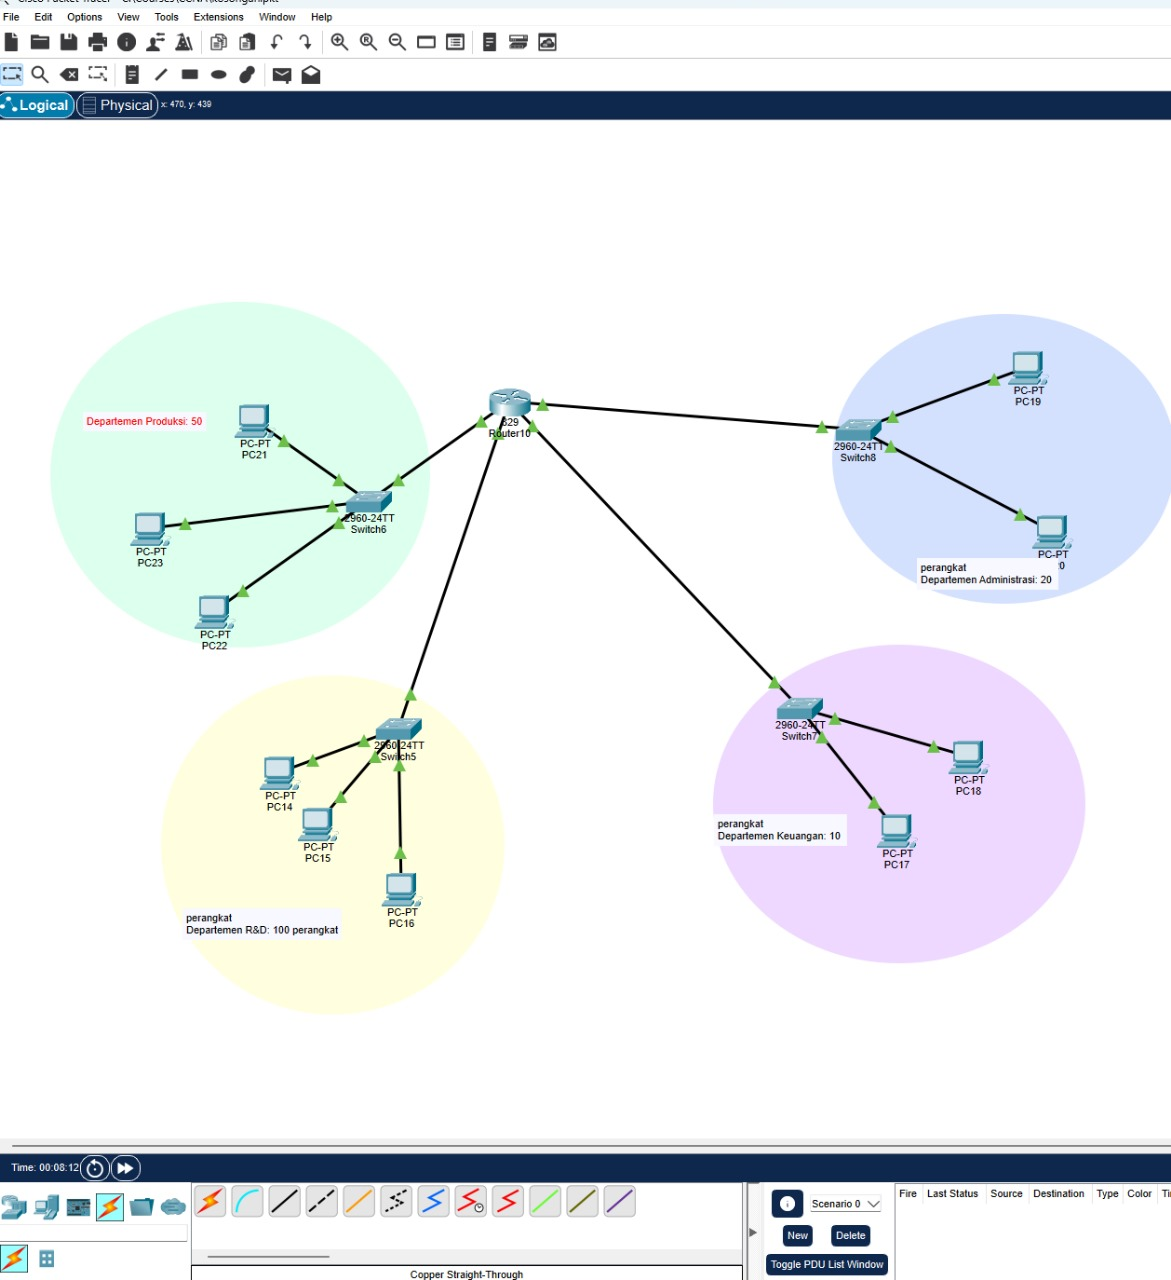
\includegraphics[width=0.5\textwidth]{Template Laporan Sementara/P1/img/WhatsApp Image 2025-05-09 at 11.30.10 AM.jpeg}
  \caption{Gambar topologi}
\end{figure}
\item Tuliskan tabel routing sederhana yang menunjukkan:
\begin{itemize}
        \item Network destination
        \item Netmask/prefix
        \item Gateway
        \item Interface tujuan
    \end{itemize}

    Jawab:
    
    Berikut adalah tabel routing yang diperlukan pada router utama:
\begin{center}
\begin{tabular}{ |c|c|c|c|c| } 
\hline
Network Destination & Netmask/Prefix & Gateway & Interface\\
\hline
92.168.0.0/26 & 255.255.255.192 & 92.168.0.1 & eth0  \\
92.168.0.64/26 & 255.255.255.224 & 92.168.0.65 & eth1  \\
92.168.0.96/26 & 255.255.255.240 & 92.168.0.97 & eth2  \\
92.168.0.112/26 & 255.255.255.128 & 92.168.0.113 & eth3  \\
\hline
\end{tabular}
\end{center}

\item Berdasarkan topologi yang telah kamu buat, jenis routing apa yang paling cocok untuk perusahaan ini? Jelaskan alasanmu secara rinci. Pilih salah satu dari opsi berikut (atau lebih jika diperlukan) dan berikan justifikasi mengapa itu menjadi pilihan terbaik untuk perusahaan ini:
\begin{itemize}
        \item Static Routing
        \item Dynamic Routing
        \item CIDR
    \end{itemize}

    jawab:
    Janis routing paling cocok adalah static routing, karena skala jaringan yang kecil dan sederhana topologi hanya melibatkan satu router saja yang dapat menghubungkan empat subnet, selain itu ideal untuk jaringan kecil karena tidak memerlukannya protokol dinamis yang kompleks untuk pertukaran informasi. Topologi ini sudah menggunakan CIDR, yang memungkinkan alokasi alamat IP yang efisien tanpa membuang alamat
\end{enumerate}